\documentclass[11pt, a4paper]{book}
\usepackage[urlcolor = blue, colorlinks = true, linkcolor = black]{hyperref}
\usepackage{graphicx}
\usepackage{fullpage}

\begin{document}
\title{Linux Guide for Chinese Beginners}
\author{Jun Sun}
\date{2014.7.7}
\maketitle
\tableofcontents\newpage

\chapter{name of chapter}
\section{name of section}
hello
\url{google.com}
\subsection{name of subsection}
This is the content
This is the content
This is the content
This is the content
This is the content
数据,是软件处理的核心,我们写各种各样的应用都是为了处理数据。

当你做某件事的时候,一旦想要求快,就表示你再也不关系它,而想去做别的事。数据,是软件处理的核心,我们写各种各样的应用都是为了处理数据。

当你做某件事的时候,一旦想要求快,就表示你再也不关系它,而想去做别的事。数据,是软件处理的核心,我们写各种各样的应用都是为了处理数据。

当你做某件事的时候,一旦想要求快,就表示你再也不关系它,而想去做别的事。

\begin{figure}[htb]
\centering
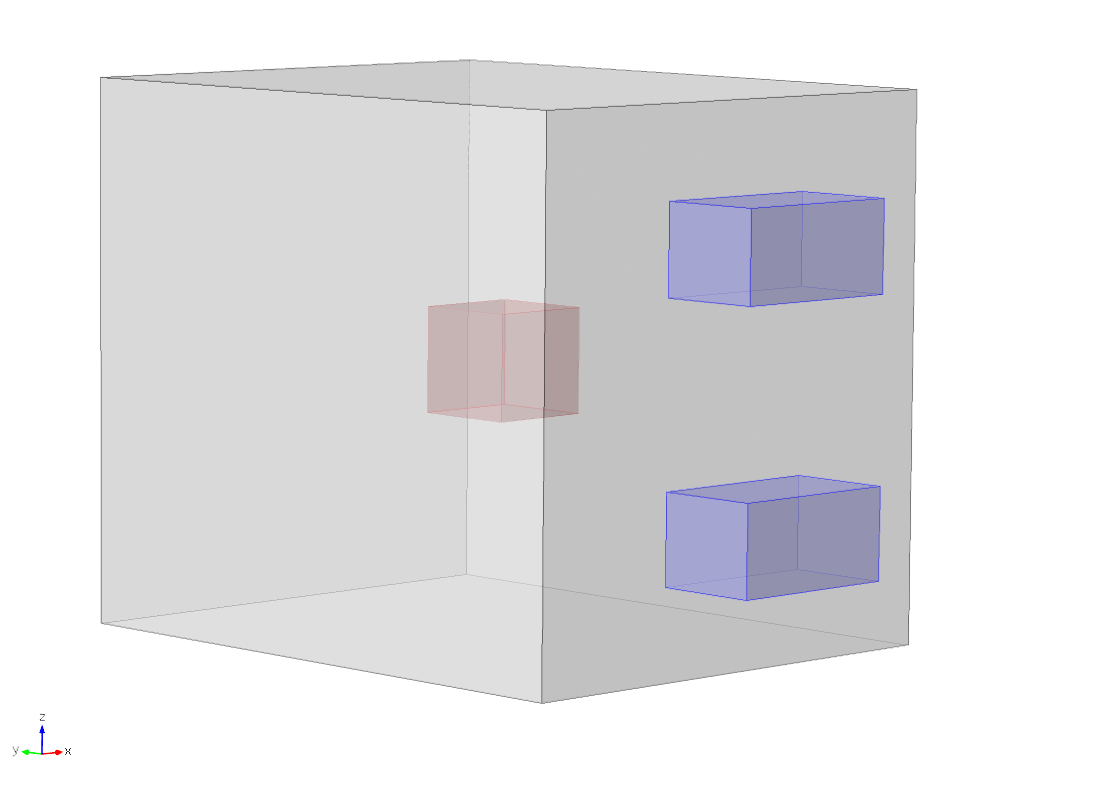
\includegraphics{./figures/two_port_model.jpg}
\caption{Local version control diagram}
\end{figure}

\chapter{name of chapter}
\section{name of section}
hello
\subsection{name of subsection}
This is the content
This is the content
This is the content
This is the content
This is the content
数据,是软件处理的核心,我们写各种各样的应用都是为了处理数据。

当你做某件事的时候,一旦想要求快,就表示你再也不关系它,而想去做别的事。数据,是软件处理的核心,我们写各种各样的应用都是为了处理数据。

当你做某件事的时候,一旦想要求快,就表示你再也不关系它,而想去做别的事。数据,是软件处理的核心,我们写各种各样的应用都是为了处理数据。

当你做某件事的时候,一旦想要求快,就表示你再也不关系它,而想去做别的事。数据,是软件处理的核心,我们写各种各样的应用都是为了处理数据。

当你做某件事的时候,一旦想要求快,就表示你再也不关系它,而想去做别的事。数据,是软件处理的核心,我们写各种各样的应用都是为了处理数据。

当你做某件事的时候,一旦想要求快,就表示你再也不关系它,而想去做别的事。数据,是软件处理的核心,我们写各种各样的应用都是为了处理数据。

当你做某件事的时候,一旦想要求快,就表示你再也不关系它,而想去做别的事。数据,是软件处理的核心,我们写各种各样的应用都是为了处理数据。

当你做某件事的时候,一旦想要求快,就表示你再也不关系它,而想去做别的事。数据,是软件处理的核心,我们写各种各样的应用都是为了处理数据。

当你做某件事的时候,一旦想要求快,就表示你再也不关系它,而想去做别的事。
\end{document}